% This is "sig-alternate.tex" V2.0 May 2012
% This file should be compiled with V2.5 of "sig-alternate.cls" May 2012
%
% This example file demonstrates the use of the 'sig-alternate.cls'
% V2.5 LaTeX2e document class file. It is for those submitting
% articles to ACM Conference Proceedings WHO DO NOT WISH TO
% STRICTLY ADHERE TO THE SIGS (PUBS-BOARD-ENDORSED) STYLE.
% The 'sig-alternate.cls' file will produce a similar-looking,
% albeit, 'tighter' paper resulting in, invariably, fewer pages.
%
% ----------------------------------------------------------------------------------------------------------------
% This .tex file (and associated .cls V2.5) produces:
%       1) The Permission Statement
%       2) The Conference (location) Info information
%       3) The Copyright Line with ACM data
%       4) NO page numbers
%
% as against the acm_proc_article-sp.cls file which
% DOES NOT produce 1) thru' 3) above.
%
% Using 'sig-alternate.cls' you have control, however, from within
% the source .tex file, over both the CopyrightYear
% (defaulted to 200X) and the ACM Copyright Data
% (defaulted to X-XXXXX-XX-X/XX/XX).
% e.g.
% \CopyrightYear{2007} will cause 2007 to appear in the copyright line.
% \crdata{0-12345-67-8/90/12} will cause 0-12345-67-8/90/12 to appear in the copyright line.
%
% ---------------------------------------------------------------------------------------------------------------
% This .tex source is an example which *does* use
% the .bib file (from which the .bbl file % is produced).
% REMEMBER HOWEVER: After having produced the .bbl file,
% and prior to final submission, you *NEED* to 'insert'
% your .bbl file into your source .tex file so as to provide
% ONE 'self-contained' source file.
%
% ================= IF YOU HAVE QUESTIONS =======================
% Questions regarding the SIGS styles, SIGS policies and
% procedures, Conferences etc. should be sent to
% Adrienne Griscti (griscti@acm.org)
%
% Technical questions _only_ to
% Gerald Murray (murray@hq.acm.org)
% ===============================================================
%
% For tracking purposes - this is V2.0 - May 2012

\documentclass{sig-alternate}

\begin{document}
%
% --- Author Metadata here ---
\conferenceinfo{ICMI}{'12 Santa Monica, California USA}
%\CopyrightYear{2012} % Allows default copyright year (20XX) to be over-ridden - IF NEED BE.
%\crdata{0-12345-67-8/90/01}  % Allows default copyright data (0-89791-88-6/97/05) to be over-ridden - IF NEED BE.
% --- End of Author Metadata ---

\title{
	{\ttlit ShEMP}: A Mobile Framework for Shared Emotion, Music, and Physiology
%		\titlenote{(Produces the permission block, and copyright information). For use with SIG-ALTERNATE.CLS. Supported by ACM.}}
%	\subtitle{[Extended Abstract]
%	\titlenote{
%		A full version of this paper is available as \textit{Author's Guide to Preparing ACM SIG 
%		Proceedings Using \LaTeX$2_\epsilon$\ and BibTeX} at \texttt{www.acm.org/eaddress.htm}
%	}
}
%
% You need the command \numberofauthors to handle the 'placement
% and alignment' of the authors beneath the title.
%
% For aesthetic reasons, we recommend 'three authors at a time'
% i.e. three 'name/affiliation blocks' be placed beneath the title.
%
% NOTE: You are NOT restricted in how many 'rows' of
% "name/affiliations" may appear. We just ask that you restrict
% the number of 'columns' to three.
%
% Because of the available 'opening page real-estate'
% we ask you to refrain from putting more than six authors
% (two rows with three columns) beneath the article title.
% More than six makes the first-page appear very cluttered indeed.
%
% Use the \alignauthor commands to handle the names
% and affiliations for an 'aesthetic maximum' of six authors.
% Add names, affiliations, addresses for
% the seventh etc. author(s) as the argument for the
% \additionalauthors command.
% These 'additional authors' will be output/set for you
% without further effort on your part as the last section in
% the body of your article BEFORE References or any Appendices.

\numberofauthors{5} %  in this sample file, there are a *total*
% of EIGHT authors. SIX appear on the 'first-page' (for formatting
% reasons) and the remaining two appear in the \additionalauthors section.
%
\author{
% You can go ahead and credit any number of authors here,
% e.g. one 'row of three' or two rows (consisting of one row of three
% and a second row of one, two or three).
%
% The command \alignauthor (no curly braces needed) should
% precede each author name, affiliation/snail-mail address and
% e-mail address. Additionally, tag each line of
% affiliation/address with \affaddr, and tag the
% e-mail address with \email.
%
% 1st. author
\alignauthor Brennon Bortz\\
       \affaddr{Institute for Creativity, Arts, and Technology}\\
       \affaddr{Virginia Polytechnic Institute and State University}\\
       \affaddr{Blacksburg, VA 24060}\\
       \email{brennon@musicsensorsemotion.com}
% 2nd. author
\alignauthor Spencer Salazar\\
       \affaddr{Center for Computer Research in Music and Acoustics}\\
       \affaddr{Stanford University}\\
       \affaddr{Stanford, California 94305}\\
       \email{spencer@ccrma.stanford.edu}
% 3rd. author
\alignauthor Javier Jaimovich\\
       \affaddr{Sonic Arts Research Centre}\\
       \affaddr{Queen's University Belfast}\\
       \affaddr{Belfast, Northern Ireland}\\
       \email{javier@musicsensorsemotion.com}
\and  % use '\and' if you need 'another row' of author names
% 4th. author
\alignauthor R. Benjamin Knapp\\
       \affaddr{Institute for Creativity, Arts, and Technology}\\
       \affaddr{Virginia Polytechnic Institute and State University}\\
       \affaddr{Blacksburg, VA 24060}\\
       \email{ben@musicsensorsemotion.com}
% 5th. author
\alignauthor Ge Wang\\
       \affaddr{Center for Computer Research in Music and Acoustics}\\
       \affaddr{Stanford University}\\
       \affaddr{Stanford, California 94305}\\
       \email{ge@ccrma.stanford.edu}
}
% There's nothing stopping you putting the seventh, eighth, etc.
% author on the opening page (as the 'third row') but we ask,
% for aesthetic reasons that you place these 'additional authors'
% in the \additional authors block, viz.

%\additionalauthors{Additional authors: John Smith (The Th{\o}rv{\"a}ld Group,
%email: {\texttt{jsmith@affiliation.org}}) and Julius P.~Kumquat
%(The Kumquat Consortium, email: {\texttt{jpkumquat@consortium.net}}).}

\date{29 June 2012}
% Just remember to make sure that the TOTAL number of authors
% is the number that will appear on the first page PLUS the
% number that will appear in the \additionalauthors section.

\maketitle
\begin{abstract}
\end{abstract}

% A category with the (minimum) three required fields
%\category{H.4}{Information Systems Applications}{Miscellaneous}
%A category including the fourth, optional field follows...
%\category{D.2.8}{Software Engineering}{Metrics}[complexity measures, performance measures]

\category{H.5.3}{Information Interfaces and Presentation}{\\Group and Organization Interfaces}[Collaborative computing, Organizational design, Synchronous interaction]
\category{H.5.2}{Information Interfaces and Presentation}{User Interfaces}[Input devices and strategies]
\category{H.5.1}{Information Interfaces and Presentation}{Multimedia Information Systems}[Audio input/output]
\category{H.5.5}{Information Interfaces and Presentation}{Sound and Music Computing}
\category{C.2.4}{Computer-Communication Networks}{Distrib\-uted Systems}[Client/server]
\category{J.5}{Arts and Humanities}[Performing arts]

\terms{Algorithms, Design, Experimentation, Measurement}

\keywords{Collaborative music, group emotion, mobile computing, physiological interfaces}

\section{Introduction}
How can we measure the quality of a creative experience?  In what ways do the emotions of participants affect or are affected by creative collaboration?  Is the perception of a musical performance altered depending on whether it is experienced individually or as a member of a group?  These are among the questions under consideration by partners, including the authors, in the Social Interaction and Entrainment using Musical Performance Experimentation (SIEMPRE) project.  Here we introduce ShEMP--a software framework through which we can explore these questions in greater depth.  ShEMP, a mobile framework for Shared Emotion, Music, and Physiology, in conjunction with MobileMuse, an unobtrusive sensor package for mobile physiological signal acquisition, leverage the distributed yet locative properties of mobile devices to allow the design of ecological experiments outside of the laboratory to investigate collaborative creativity and shared experience of musical performances.  This paper provides a brief introduction to several notable advances made in recent and current SIEMPRE experiments that have been particularly motivating to the development of ShEMP.  This is followed by an overview of the design of ShEMP and a discussion of the suite of technologies it employs.  We then elaborate on an initial battery of experiments to be executed presently, for which the framework was designed.

\section{Background}
For the last two years, the Social Interaction and Entrainment using Music Performance Experimentation (SIEMPRE) project has focused on measuring interpersonal creative interaction on the backdrop of music performance.  The experiments designed and executed thus far have focused on these the experience of musical performance and experience in the following interconnected areas (\cite{SIEMPREProjectConsortium:2011vh}):

\begin{itemize}
	\item Musician/musician interactions
	\item Conductor/musicians interactions
	\item Music/listener interactions
	\item Musician/listener interactions
\end{itemize}

Within these scenarios, our attention is drawn to four different foci: \textit{entrainment}, and \textit{emotional contagion}, \textit{co-creation}, and \textit{leadership}.  The first of these, entrainment, is described by Clayton, Sager, and Will (\cite{Clayton:2005wc}) as ``a process whereby two rhythmic processes interact with each other in such a way that they adjust towards and eventually `lock in' to a common phase and/or periodicity.''  This takes shape on multiple levels and in various situations: from a listener's foot tapping in tempo with music or their respiration and heart rates coming into synchronization (albeit often much more slowly) with the beat of the music, to an organisms internal physiological processes' entrainment to one another, or to those of another organism within a group.  Indeed, as Clayton, Sager, and Will note, humans' internal rhythmic processes can and do entrain to both other internal rhythms as well as to those of other humans through music performance and shared experience of music.  This potential for entrainment through social interaction by way of music is of particular interest to SIEMPRE.

Closely linked to entrainment is emotional contagion.  In their seminal work on the subject, Hatfield, Cacioppo, and Rapson (\cite{Hatfield:1994us}) describe the phenomenon of emotional contagion as one in which a particular emotional episode in one individual can evoke stimuli that act upon other individuals to bring about similar or complementary emotional responses.  While the related phenomenon, empathy, requires cognitive and autonomic facility, Hatfield et al. argue that emotional contagion is an automatic and involuntary process.  Converse to empathy, they further define contagion as a process in which humans automatically mimic and synchronize the behaviors of another, and as a result, converge emotionally (\cite{Hatfield:1992us}).  Emotional contagion not only strengthens emotional bonds between people, however; the presence and awareness of emotional contagion in interpersonal interaction affects meaning and significance in communication, aid in understanding social interaction, and facilitate empathy and sympathy, for instance.  It is this significance that places emotional contagion as the second focus of SIEMPRE's research into interpersonal interaction.

Several studies under the SIEMPRE umbrella are concerned with musical co-creation.  This is not necessarily completely bound up in musical performance by expert musicians, but includes the idea that audience and performer alike work together to shape a performance.  On the one hand, performance process is informed not only by the training and preparation of the musician, for instance, but also by their awareness of and response to input, active or otherwise, from the audience.  On the other hand, co-creation also occurs where novice musicians work together to create music for only themselves to experience.  In either case, and in all those in between, co-creation serves to bind the group socially and serves as another means for social interaction.

The final focus within interaction that concerns SIEMPRE is leadership.  Here again, a common paradigm in musical performance parallels that of everyday human interaction.  By varying manipulating the leadership role, we can examine not only how changes to leadership affect group interaction in general, but also the specific implications these changes may have such already discussed phenomena as synchronization and entrainment, and the emotional understanding of the audience and performers.

\section{Recent Work and Motivations}
With this as the focus, SIEMPRE partners have designed and executed a wide array of experiments both within and without the SIEMPRE umbrella.

\vspace{12pt}
\textbf{\textit{Overview of notable experiments and results here...  Recent work and/or motivations from CCRMA and Javier...}}
\vspace{12pt}

\subsection{Emotion in Motion}
Emotion in Motion is an ongoing research project, investigating people�s affective response to musical stimuli in non-laboratory environments. The aim of this study is to explore the relationship between the musical content and changes in the emotional response of the listener, via physiological measurements and self-report questionnaires.

The data capture terminal was designed as an installation that can operate in a public gallery or science centre (see Figure~\ref{fig:eyebeam}), where participants can take part in the experiment without external assistance by following on-screen instructions. Even though there have been several iterations and changes to the experimental design, the experiment consists essentially in the participant answering a small number of background and demographic questions (e.g. age, gender, musical expertise, etc.), and then listening to an approximately 90-second long musical excerpt selected randomly from a pool of songs of diverse styles, eras and emotional intent. While the music is playing, two physiological measurements are recorded simultaneously: electrodermal activity (EDA) and heart rate (HR). EDA and HR were chosen for their acknowledged use as physiological indicators of emotion (PIE) in the psychophysiology literature (see \cite{Plutchik:1994we}, \cite{Cacioppo:2000ws}, \cite{Jaimovich:2010wr}, and \cite{Boucsein:2011ub}), as well as for their unobtrusive measurement (both can be captured with sensors worn on one hand). After the excerpt completes, participants are asked to answer a brief self-report questionnaire, indicating how the music made them feel, their level of engagement and enjoyment, among other questions. This process is repeated for three different excerpts. For a detailed description of the experimental design, please refer to \cite{Jaimovich:2012vr}.

\begin{figure}[h]
	\centering
	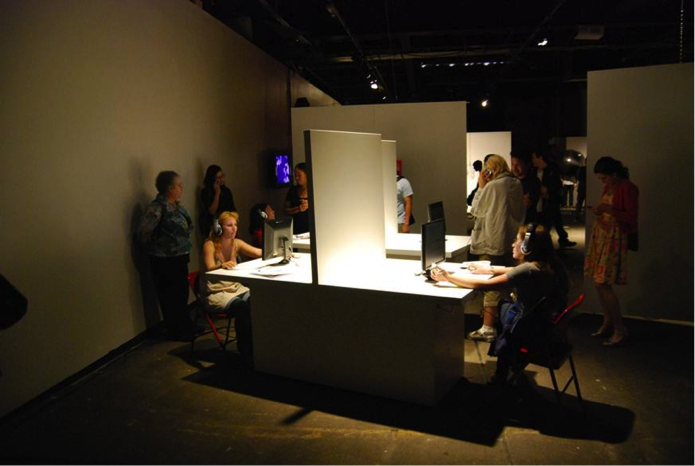
\includegraphics[width=\linewidth,angle=0,keepaspectratio=true,trim=0 0 0 0,clip=true]{eyebeam}
	\caption{Participants at the Eyebeam Gallery in New York City, June 2011.}
	\label{fig:eyebeam}
\end{figure}

The first iteration of the experiment started in the Science Gallery, Dublin, where it ran for a period of three months in the summer of 2010, having been later installed in public galleries in New York City, Genova, and currently running in Bergen and Singapore. To the date of this submission, over 6000 people have participated in the experiment, having more than 18000 recordings of physiological data associated with a musical excerpt. 

Even though the greater part of the work conducted to this point has been focused in improving the data acquisition and feature extraction of signals, preliminary results show a significant correlation between physiological features and the self-reported questionnaire (\cite{Jaimovich:2012vr}). A detailed discussion of the experiment�s results is beyond the scope of this paper. Nonetheless, while analyzing the Emotion in Motion database, several mitigating factors were found that influence changes in physiology. We believe that these factors need to be taken into account when designing interfaces that use changes in physiology as measures of emotion.

\subsection{Motivation}
Several studies, particularly those with a focus on audience experience of music--be it a live performance, a video recording of a live performance, audio of a studio recording, or otherwise--note the importance of observing the audience experiment in as ecological a manner as possible (see \cite{Jaimovich:2012vr}, for example).  Furthermore, it is at least presumable that a good deal, if not the majority, of an individual's time spent experiencing music is when they are either alone, or among a small group of people--not in either a concert hall or laboratory.  Issues of ecological validity aside, it is at least important to consider implications on the aforementioned research foci when audiences (of one or more) experience music individually.

In 2012, SIEMPRE established an International Cooperation project (SIEMPRE-INCO) to explore these areas in further detail.  Specifically, the SIEMPRE-INCO project addresses empathic processes within the aforementioned four areas of interaction, but in remote locations.  It aims at understanding how emotional contagion and co-creation can and do occur when the individuals or audiences who are participating do not share the same physical environment.  How is the experience shaped the when two people share a listening experience from two different locations?

\section{ShEMP Design and Implementation}
To explore the questions of SIEMPRE-INCO, we have built ShEMP, a framework upon which we can construct a range of experimental apparatuses.  A great deal of the partners' previous work has served to determine or the efficacy of a range of measure of audience (interactor) response mechanisms, including self-report questionnaires, input based around the GEMS scale, and judgements.  ShEMP's flexibility allows us to collect voluntary feedback using any or a combination of these models with ease.  Coupled with this, the MobileMuse sensor provides ShEMP participant physiological data--pulse oximetry, electrodermal activity, motion, and skin temperature.  This section discusses the software and hardware design and implementation of ShEMP.

\subsection{Software}
\vspace{12pt}
\textbf{\textit{Your space, Spencer.}}
\vspace{12pt}

\subsubsection{Digital Signal Processing}
In order to allow the hardware to interface with a variety of devices, signal is passed over a standard 1/8'' (3.5mm) TRRS audio plug, as the 1/8'' TRRS audio jack has become all but the standard on consumer mobile devices.  However, as standard wiring uses only the sleeve of the TRRS plug for input, it was necessary to devise a way to receive multiple input signals over a single channel.  On the mobile device (currently iOS devices are supported), the signal is received as an audio input stream.  Within Apple's AudioUnit framework, the passes through a DSP chain in order to split the multiplexed signal back into its original constituent signals.

The signal is first lowpass-filtered (\(Fc = 7.5 \text{kHz}\)) in order to remove noise introduced by pulse-width modulation from the sensor hardware.  The signal is then multiplied sample-by-sample with sine waves at the frequencies of the component carrier waves established in frequency-division multiplexing in the sensor circuit.  In order to address frequency and phase jitter introduced by pulse-width modulation and timer imprecision from in the sensor micro-controller unit, a phase-lock loop is established between the filtered incoming signal and software oscillators controlled by the demodulation routine.  These multiplications produce sine waves with a positive DC offset at double the frequency of the initial carrier waves for each component signal.  These signals are then further lowpass-filtered (\(Fc = 25 \text{Hz}\)) to remove said sine waves and leave only the slowly varying DC offset as the final demodulated output for each signal.  These demodulated outputs are then exposed to other components of the framework for recording, streaming to an external server, sharing with other devices, or visualization within the user interface.

\subsection{Hardware}
It was decided that the entire sensor system must fit on a single finger. In order to accomplish this, heart rate is measured using standard pulse oximetry techniques rather than a full electrocardiogram. The MobileMuse board (\cite{Knapp:2011vl}) houses four discrete sensors. Upon further consideration, and because of the ease of design, a temperature sensor was also added to the interface. Skin temperature change (in relationship to the environment) has been shown to be indicative of long term mood and it is thought that this might prove beneficial in assessment of emotional state. A triaxial accelerometer was also added to the circuit for gestural control. While this might seem redundant, independent hand gesture might introduce interesting options not presently available with a mobile device's onboard accelerometer or gyroscope. At minimum this enables two-handed gestural control.  Furthermore, an independent accelerometer provides a means of minimizing motion artifacts, an issue to which EDA sensors are particularly susceptible.

As shown in the block diagram in Figure 5, all of the sensor signals are amplified, processed, conditioned and then fed into the ADCs of an ATMega328PU processor. The choice of this process enables use of the MobileMuse as a custom Arduino board with all of the advantages this creates---most importantly, ubiquitous software availability. The ATMega processor firmware frequency-division multiplexes the sensor signals in order to create one single audio data stream for ease of transmission over the sleeve of the TRRS plug. The signal is then reconverted to an analog stream using the pulse-width modulation (PWM) output of the processor fed through an onboard DAC. Finally, magnetic isolation is used to remove any shock risks and to eliminate line noise.

\section{Proposed Sequence of Experiments}
Taking the progress made in the Emotion in Motion experiments (\cite{Jaimovich:2012vr}) as a starting point, we propose a battery of experiments to explore group emotion, emotional contagion, and co-creation in a mobile environment.  In particular, these experiments aim to answer the following questions:

\begin{itemize}
	\item How does the psychophysiology of a listener as a part of a group differ from when they listen alone?
	\item Does a listener's simple awareness that a listening or creative exercise is collaborative alter their emotional response?
	\item What representations of this collaboration are most conducive to emotional contagion?
	\item Does a listener's awareness that a listener or creative exercise is collaborative alter their \textit{quality of experience}? (\cite{SIEMPREProjectConsortium:2011vh}, \cite{SIEMPREProjectConsortium:2012tj})
	\item Does a participant's awareness of their remote collaborator's emotional state(s) affect the quality of experience of collaborative music making?
\end{itemize}

To this end, we propose a sequence of iterative experiments that leverage ShEMP.  In the first experiment, each participant will be equipped with a mobile phone and MobileMuse sensor.  Background (including musical) and demographic information will be gathered from each participant.  When a case commences, the participant will be paired with a participant in a geographically separate location.  The two participants will be streamed selections of music drawn from the pool of songs with validated emotional content from the Emotion in Motion experiment.  Following each song selection, participants will be guided through a self-response questionnaire regarding their quality of experience.  The design of this questionnaire will be tuned based on recent results from Emotion in Motion and other SIEMPRE work around quality of experience.  Throughout the process, physiological data from each participant will be captured through the attached MobileMuse.

Our initial hypothesis is that a listener's simple awareness that a listening experience is collaborative will affect their emotional response.  Assuming that this hypothesis holds, the sequence of experiments will continue to explore ways to improve the collaborators' quality of experience and to make such an interaction further conducive to emotional contagion.  This will be explored in successive experiments in the following ways:

\begin{itemize}
	\item Presentation of collaborator's physiological data streams to the listener in real time
	\item Presentation various visualizations of collaborator's emotional response through shadow media (REF: Miwa/shadow media)
	\item Enabling interaction with a group of collaborators selected by the participant based on demographic, location, musical selection, etc.
\end{itemize}

If our initial hypothesis does not hold, we intend to approach the successive experiments with the aim of reshaping our initial hypothesis---seeking ways in which a shared musical experience across remote locations can indeed affect their emotional response, enhancing emotional contagion and improving quality of experience.

\section{Potential Issues}
\vspace{12pt}
\textbf{\textit{Anyone feel free to chime in here...}}
\vspace{12pt}

\section{Final Remarks}

%\end{document}  % This is where a 'short' article might terminate

%ACKNOWLEDGMENTS are optional
\section{Acknowledgments}
The project SIEMPRE acknowledges the financial support of the Future and Emerging Technologies (FET) programme within the Seventh Framework Programme for Research of the European Commission, under FET-Open grant number: 250026-2.

%
% The following two commands are all you need in the
% initial runs of your .tex file to
% produce the bibliography for the citations in your paper.
\bibliographystyle{abbrv}
\bibliography{ICMI_Paper_References}
% You must have a proper ".bib" file
%  and remember to run:
% latex bibtex latex latex
% to resolve all references
%
% ACM needs 'a single self-contained file'!
%
%APPENDICES are optional
%\balancecolumns
%\balancecolumns % GM June 2007
% That's all folks!
\end{document}
